\documentclass{standalone}
\usepackage{picture,color}
\usepackage{graphicx}
\graphicspath{{./scan_1_raw/}}
\setlength{\unitlength}{1in}
\renewcommand{\rmdefault}{phv} % Arial
\renewcommand{\sfdefault}{phv} % Arial

\begin{document}
\begin{picture}(7.1, 3.26)(0.04,-4.79)

% example neurons 
\linethickness{0.01in}
%% cell 1-5
\put(0.18, -1.9){
\includegraphics[height=0.35in]{em_example_1_4.pdf}}
\put(0.18, -2.2){
\includegraphics[height=0.35in]{2p_example_1_4.pdf}}
\put(0.09, -1.825){\rotatebox{90}{\small EM}}
\put(0.09, -2.125){\rotatebox{90}{\small 2P}}
\multiput(0.061, -2.17)(0, 0.62){2}{\color{black}\line(1, 0){7.05}}
\multiput(0.061, -2.17)(7.05,0){2}{\color{black}\line(0, 1){0.62}}

% \put(3.29, -1.45){Example spatial footprints}
% cell 6-10 
\put(0.18, -2.55){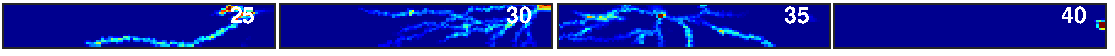
\includegraphics[height=0.35in]{em_example_5_8.pdf}}
\put(0.18, -2.85){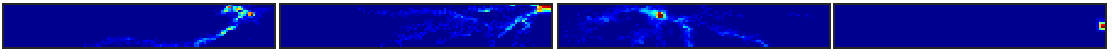
\includegraphics[height=0.35in]{2p_example_5_8.pdf}}
\multiput(0.061, -2.82)(0, 0.62){2}{\color{black}\line(1, 0){7.05}}
\multiput(0.061, -2.82)(7.05,0){2}{\color{black}\line(0, 1){0.62}}
\put(0.09, -2.475){\rotatebox{90}{\small EM}}
\put(0.09, -2.775){\rotatebox{90}{\small 2P}}
 
% cell 11-15 
\put(0.18, -3.2){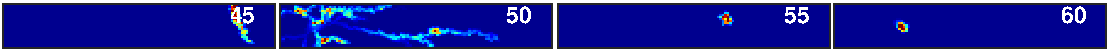
\includegraphics[height=0.35in]{em_example_9_12.pdf}}
\put(0.18, -3.5){
\includegraphics[height=0.35in]{2p_example_9_12.pdf}}
\multiput(0.061, -3.47)(0, 0.62){2}{\color{black}\line(1, 0){7.05}}
\multiput(0.061, -3.47)(7.05,0){2}{\color{black}\line(0, 1){0.62}}
\put(0.09, -3.12){\rotatebox{90}{\small EM}}
\put(0.09, -3.42){\rotatebox{90}{\small 2P}}

% cell 16-20
\put(0.18, -3.85){
\includegraphics[height=0.35in]{em_example_13_16.pdf}}
\put(0.18, -4.15){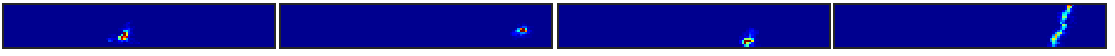
\includegraphics[height=0.35in]{2p_example_13_16.pdf}}
\multiput(0.061, -4.12)(0, 0.62){2}{\color{black}\line(1, 0){7.05}}
\multiput(0.061, -4.12)(7.05,0){2}{\color{black}\line(0, 1){0.62}}
\put(0.09, -3.77){\rotatebox{90}{\small EM}}
\put(0.09, -4.12){\rotatebox{90}{\small 2P}}

\put(0.18, -4.5){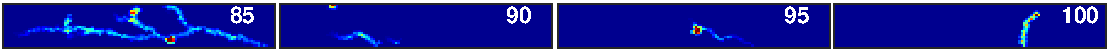
\includegraphics[height=0.35in]{em_example_17_20.pdf}}
\put(0.18, -4.8){
\includegraphics[height=0.35in]{2p_example_17_20.pdf}}
\multiput(0.061, -4.77)(0, 0.62){2}{\color{black}\line(1, 0){7.05}}
\multiput(0.061, -4.77)(7.05,0){2}{\color{black}\line(0, 1){0.62}}
\put(0.09, -4.42){\rotatebox{90}{\small EM}}
\put(0.09, -4.72){\rotatebox{90}{\small 2P}}

\end{picture}
\end{document}\grid
